%----------------------------------------------------------------------------
%----------------------------------------------------------------------------
The interaction table begins with the final stage of conditioning: spectral filtering. The spectral filter is an etalon with a FSR $<$ 3GHz (to prevent aliasing) and mode widths ranging from 100 MHz (for long pulse experiments) to 552 MHz (for short pulse experiments). The beam line presented here assumes planar etalons - some redesign will be required if confocal etalons are used. See figure \ref{interaction_mileposts}.
%----------------------------------------------------------------------------
% interaction_table_mileposts.tex
% by Troy Hix, May 2005
%----------------------------------------------------------------------------
\begin{sidewaysfigure}
\center
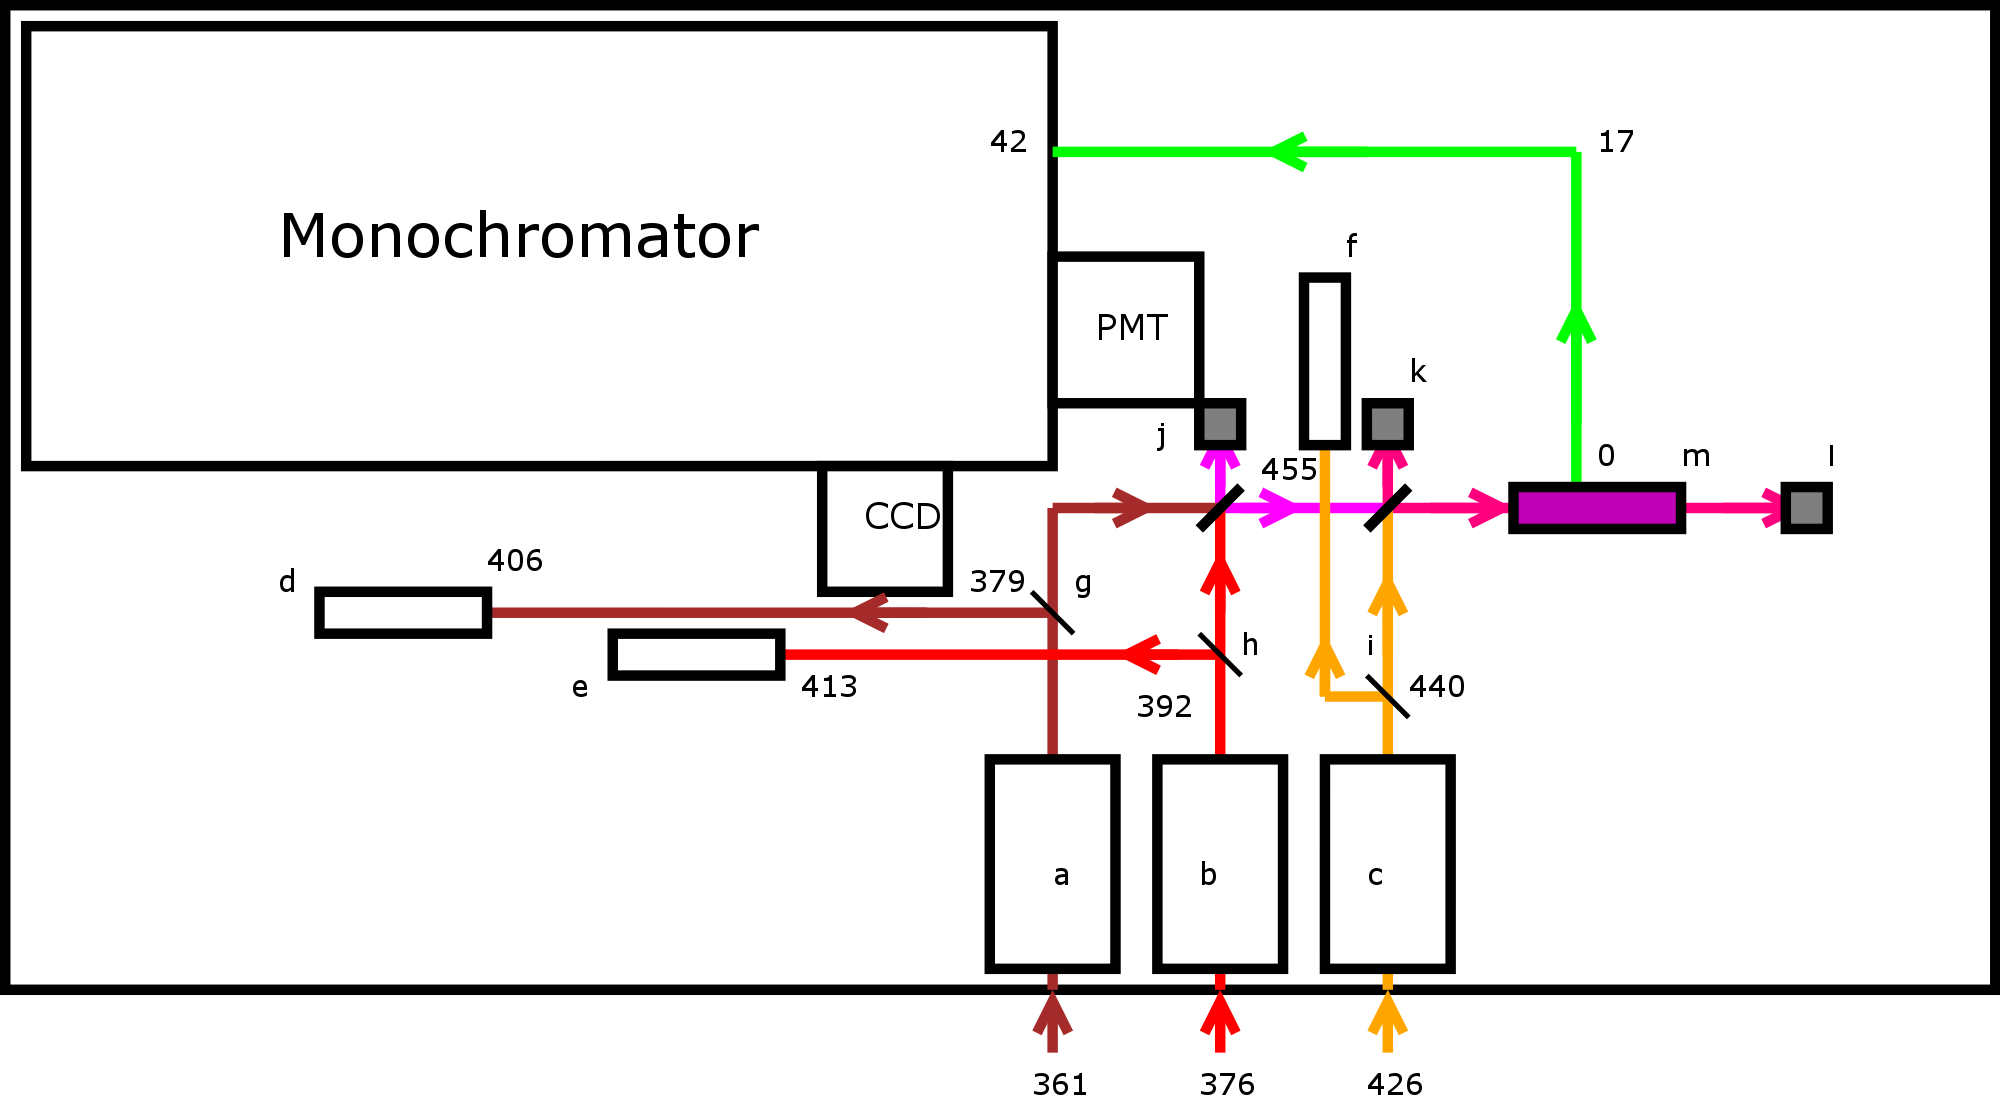
\includegraphics[width=7.75in]
{interaction_mileposts/interaction_mileposts.png}
\caption[Interaction table beam mileposts and optical component labels]{Interaction table beam mileposts and optical component labels. There is a 6X8 inch foot print for the etalons (a), (b), and (c). (d),(e), and (f) are the energy meters and pinholes for each beam. (g) is a pick-off placed at milepost 379 along the beam from dye laser \#23 - similarly for (h) and (i). (j), (k), and (l) are beam dumps and (m) is the iodine cell and its pinhole.}
\label{interaction_mileposts}
\end{sidewaysfigure} 
%----------------------------------------------------------------------------
%----------------------------------------------------------------------------
%----------------------------------------------------------------------------



%----------------------------------------------------------------------------

The three dye laser beams are then mixed using beam splitters. Once the beam are collinear, they are incident upon a pinhole placed just upstream from the iodine cell. Pick-offs are placed before the beams splitters to sample each input beam. Energy detectors are placed downstream from the pick-offs so that they are at the same beam milepost as the iodine cell. Duplicate pinholes are placed upstream from each detector; identical to the iodine cell's pinhole. Figure \ref{interaction_positions} shows the beam positions required.
%----------------------------------------------------------------------------
% interaction_table_positions.tex
% by Troy Hix, May 2005
%----------------------------------------------------------------------------
\begin{sidewaysfigure}
\center
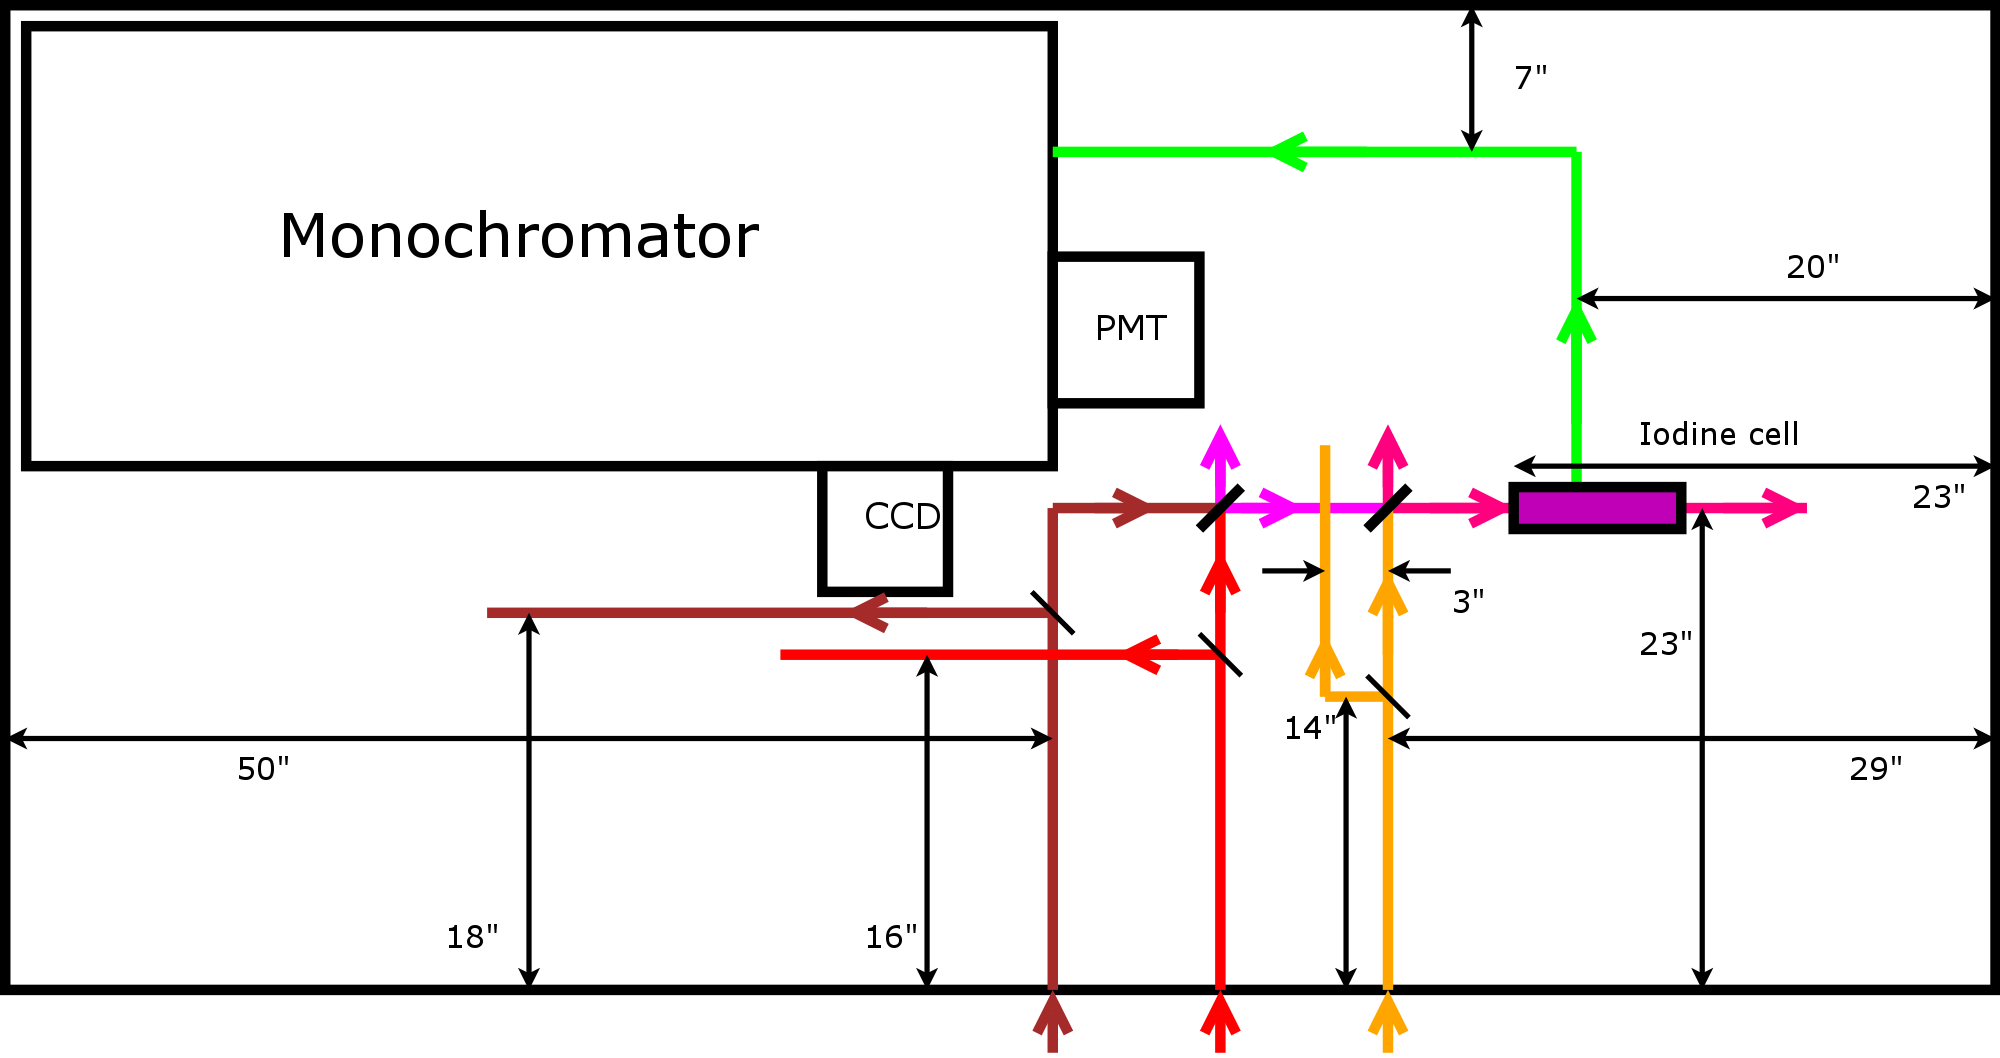
\includegraphics[width=7.75in]
{interaction_positions/interaction_positions.png}
\caption[Interaction table beam positions]{Interaction table beam positions. The mixed beams are shown in light pink and dark pink, the green beam is the fluorescence signal.}
\label{interaction_positions}
\end{sidewaysfigure} 
%----------------------------------------------------------------------------
%----------------------------------------------------------------------------
%----------------------------------------------------------------------------



%----------------------------------------------------------------------------


In figure \ref{interaction_mileposts} we see that the beam from dye laser \#21 traveled 413 inches to reach the energy detector labeled (e) in the figure. This is the same distance the beam travels to reach the iodine cell labeled (m). If we add the distance the YAG beam traveled to pump dye laser \#21 we obtain 503 inches. It can be shown using figures \ref{dye_mileposts} and \ref{interaction_mileposts} that the other two dye lasers have this same sum. Thus, assuming the path lengths inside each dye laser is the same, we conclude the three pulses arrive at the iodine cell (and the energy detectors) simultaneously.
%----------------------------------------------------------------------------
% dye_table_mileposts.tex
% by Troy Hix, May 2005
%----------------------------------------------------------------------------
\begin{sidewaysfigure}
\center
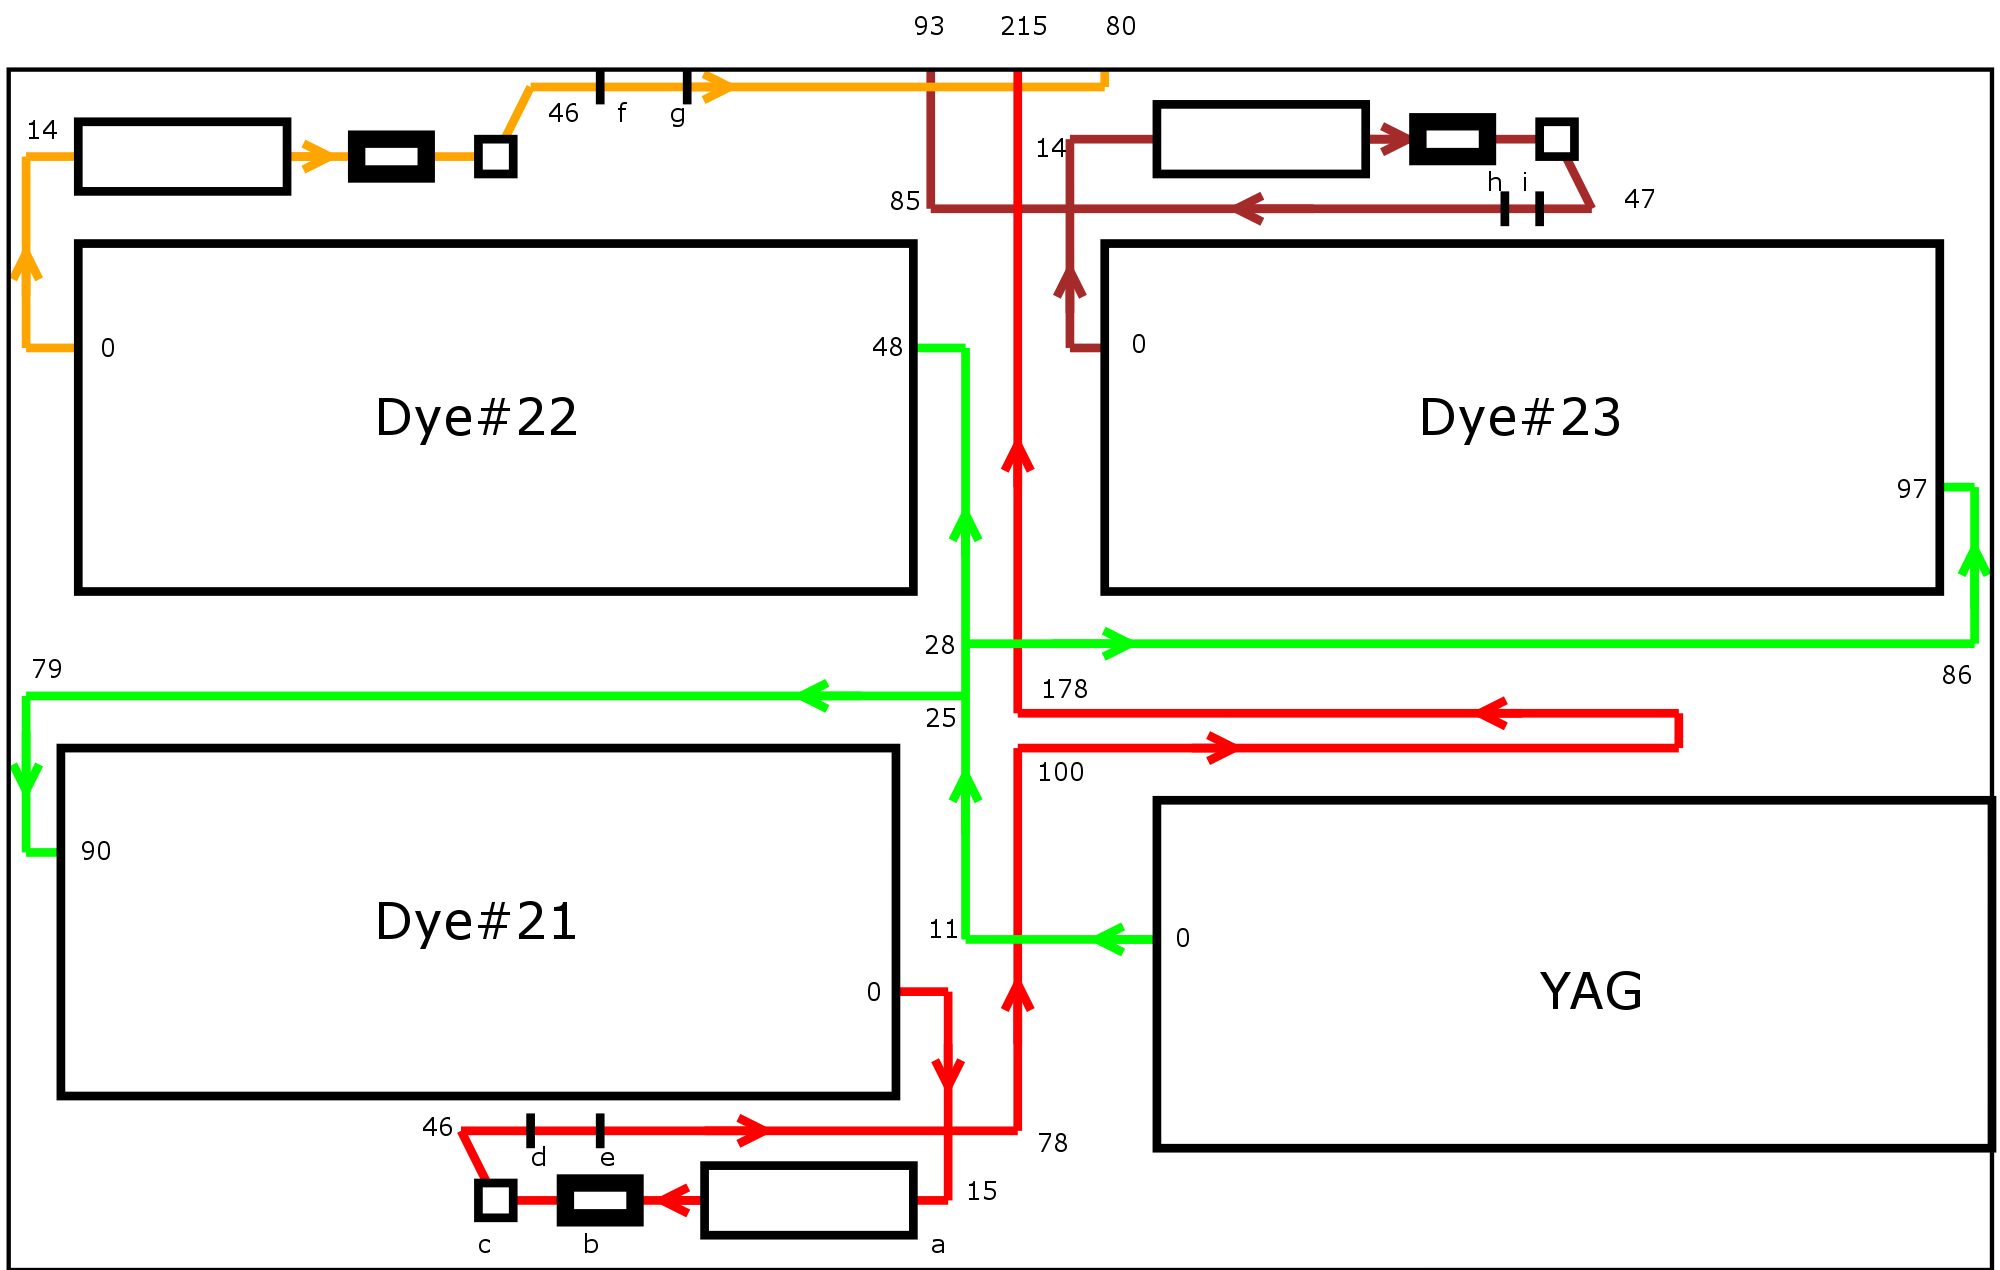
\includegraphics[width=7.75in]
{dye_mileposts/dye_mileposts.png}
\caption[Beam mileposts and optics on the dye laser table]{Beam mileposts and optics on the dye laser table. the mileposts along each beam line is given in inches. Optic (a) is a pile-of-plates polarizer; (b) Pockels cell, (c) Brewster plate, (d) +1 m lens at mile post 50, (e) -1 m lens at milepost 54, (f) +1 m lens at milepost 50, (g) -1 m lens at milepost 55, (h) +1 m lens at milepost 50, (i) -1 m lens at milepost 52.5.}
\label{dye_mileposts}
\end{sidewaysfigure} 
%----------------------------------------------------------------------------
%----------------------------------------------------------------------------
%----------------------------------------------------------------------------



%----------------------------------------------------------------------------
%----------------------------------------------------------------------------
%----------------------------------------------------------------------------
%----------------------------------------------------------------------------
%----------------------------------------------------------------------------
